\documentclass{exam}
\usepackage{../../mypackages}
\usepackage{../../macros}

\setlength{\parindent}{0pt}

\title{Correction - Interro N°1 - Masse volumique + Atome}
\author{N. Bancel}
\date{3 Octobre 2024}

\begin{document}

\textbf{Collège Lycée Suger}
\hfill
\textbf{Physique-Chimie} \\

\textbf{Année 2024-2025}
\hfill
\textbf{3ème Cambridge International} \par

{\let\newpage\relax\maketitle}

\begin{center}
\textbf{\textcolor{red}{Correction}}
\end{center}

\section*{Masse volumique}

\begin{questions}
  \question[0.5] \textbf{Définir rapidement ce que signifie "l'unité légale dans le système international".}

  L'unité légale dans le système international (SI) est l'unité standard utilisée pour mesurer une grandeur physique. Elle est définie par une convention internationale pour garantir l'uniformité des mesures. Chaque grandeur physique possède une unité spécifique dans le SI.

  Exemples :
  \begin{itemize}
    \item La masse : \si{kg} (kilogramme)
    \item La longueur : \si{m} (mètre)
    \item Le temps : \si{s} (seconde)
    \item L'intensité électrique : \si{A} (ampère)
    \item L'énergie : \si{J} (joule)
    \item La force : \si{N} (newton)
  \end{itemize}
  Ces unités sont utilisées mondialement afin de faciliter les échanges scientifiques et techniques entre pays.

  \question[1] \textbf{Quelle est l'expression de la masse volumique d'un matériau ? Préciser les unités légales dans le système international de chaque variable.}

  La masse volumique, notée $\rho$, est donnée par la formule :
  \[
  \rho = \frac{m}{V}
  \]
  où $m$ est la masse (en kilogrammes, \si{kg}) et $V$ est le volume (en mètres cubes, \si{m^3}). La masse volumique s'exprime en kilogrammes par mètre cube (\si{kg/m^3}).

  Exemple : L'eau a une masse volumique de \SI{1000}{kg/m^3}, tandis que l'air a une masse volumique d'environ \SI{1.2}{kg/m^3}. Ces différences influencent les propriétés de flottabilité, par exemple.

  \question[1] \textbf{Formules déduites}

  \begin{itemize}
    \item Si l'on dispose de la valeur du volume $V$ et de la masse volumique $\rho$, la masse $m$ est donnée par :
    \[
    m = \rho \times V
    \] \par
    Exemple : Si un volume de \SI{2}{m^3} d'eau a une masse volumique de \SI{1000}{kg/m^3}, alors la masse de l'eau est :
    \[
    m = 1000 \times 2 = 2000\,\si{kg}
    \]
    \item Si l'on dispose de la masse $m$ et de la masse volumique $\rho$, le volume $V$ est donné par :
    \[
    V = \frac{m}{\rho}
    \] \par
    Exemple : Pour une masse de \SI{500}{kg} de plomb avec une masse volumique de \SI{11340}{kg/m^3}, le volume est :
    \[
    V = \frac{500}{11340} \approx 0.044\,\si{m^3}
    \]
  \end{itemize}

  \question[2] \textbf{La masse volumique du sable est de \SI{1850}{kg/m^3} en moyenne. Pour un chantier, une entreprise de maçonnerie a besoin de \SI{50}{tonnes} de sable.}

  \begin{itemize}
    \item \textcolor{blue}{\textbf{Indication :} $\frac{50}{18.5} \approx 2.702$ et $\frac{60.2}{21} \approx 2.866$}
    
    \item \textbf{Peut-elle transporter tout le sable dans un camion benne de \SI{21}{m^3} ? Pourquoi ?}

    La masse volumique étant de \SI{1850}{kg/m^3}, le volume nécessaire pour transporter \SI{50}{tonnes} (ou \SI{50000}{kg}) est :

    \[
    V = \frac{50000}{1850}
    \]

    En divisant par 100 en haut et en bas, on s'aperçoit que :

    \[
    V = \frac{500}{18.5} = \frac{50}{18.5} \times 10
    \]

    La valeur de \(\frac{50}{18.5}\) nous est donnée dans l'énoncé, donc :

    \[
    V \approx 2.702 \times 10 = 27.02\,\si{m^3}
    \]

    Ainsi, le volume nécessaire est environ \SI{27.02}{m^3}, ce qui est supérieur à la capacité du camion (\SI{21}{m^3}). Un seul camion ne suffit donc pas à transporter tout le sable.
    \item Si l'on suppose que le 1er camion a été intégralement rempli de sable, quel est le \% de remplissage du 2ème camion ?
    
    Si le premier camion est rempli à \SI{21}{m^3}, le volume restant à transporter est :
    \[
    V_{\text{reste}} = 27.02 - 21 = 6.02\,\si{m^3}
    \]
    Si le deuxième camion a une capacité de \SI{21}{m^3}, le pourcentage de remplissage du 2ème camion sera :
    \[
    \text{\% remplissage} = \frac{6.02}{21} = \frac{6.02}{21} \times \frac{10}{10} = \frac{60.2}{21} \times \frac{1}{10}
    \]
    
    La valeur de \(\frac{60}{21}\) nous est donnée dans l'énoncé, donc :

    \[
      \text{\% remplissage} = \frac{2.8666}{10} \approx 0.2871 
    \]

    Le 2ème camion est donc rempli à $\approx 28.71\%$
    
  \end{itemize}

  \question[2] \textbf{Effectuer les conversions suivantes :}

  Dans cette question sur les conversions, il est important de faire 2 choses :

  \begin{enumerate}
    \item Quand c'est possible, remettre ces dimensions dans le contexte de la vie réelle : une canette de coca fait 33cL, on voit cette unité au quotidien. Il est facile de se dire que 3 canettes font 1L. Ce sont des ordres de grandeur auxquels nous sommes habitués.
    \item Quand on travaille avec des unités sous forme de fraction (type $kg/m^3$), on raisonne aussi avec les fractions pour faire les conversions
  \end{enumerate}

  \begin{itemize}
    \item \SI{1}{kg} = \SI{1000}{g}
    \item \SI{1}{L} = \SI{100}{cL} = \SI{1000}{mL}
    \item \SI{1}{m^3} = \SI{1000}{dm^3} = \SI{1000}{L}
    \item \SI{1}{kg/m^3} = \SI{1}{g/L}
  \end{itemize}

Justification pour la conversion de $kg/m^3$ à $g/L$ : $1 kg = 1000 g$ et $1 m^3 = 1000 L$ donc 

\[
  \SI{1}{kg/m^3} = \frac{\SI{1}{\kilogram}}{\SI{1}{\cubic\meter}} = \frac{\SI{1000}{g}}{\SI{1000}{L}} = \SI{1}{g/L}
\]

\end{questions}

\section*{L'atome}

\begin{questions}
  \question[1] \textbf{A partir du schéma ci-dessous, remplir les légendes (1), (2), (3). Quel est le nom plus global pour les particules (2) et (3) ?}

  \begin{figure}[H]
    \centering
    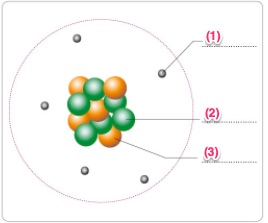
\includegraphics[width=0.6\linewidth]{interro1_01.jpg}
    \caption{\label{} Structure de l'atome}
  \end{figure}

  \begin{itemize}
    \item (1) : Noyau de l'atome
    \item (2) : Proton
    \item (3) : Neutron
  \end{itemize}
  Les protons et les neutrons sont appelés des nucléons, car ils sont présents dans le noyau de l'atome.

  \question[1] \textbf{Un atome est souvent symbolisé par le schéma ci-dessous. Que signifient $A$, $X$, et $Z$ ?}

  \begin{figure}[H]
    \centering
    
\includegraphics[width=0.3\linewidth]{interro1_02.jpg}
    \caption{\label{} Symbole de l'atome}
  \end{figure}

  \begin{itemize}
    \item $X$ : Symbole de l'élément
    \item $A$ : Nombre de masse (nombre total de protons et de neutrons)
    \item $Z$ : Numéro atomique (nombre de protons)
  \end{itemize}

  \begin{itemize}
    \item \textbf{Hydrogène} : $_{1}^{1}\text{H}$
    \begin{itemize}
        \item $X = \text{H}$ (symbole de l'élément)
        \item $A = 1$ (nombre de masse, 1 proton)
        \item $Z = 1$ (numéro atomique, 1 proton)
    \end{itemize}

    \item \textbf{Carbone} : $_{6}^{12}\text{C}$
    \begin{itemize}
        \item $X = \text{C}$ (symbole de l'élément)
        \item $A = 12$ (6 protons et 6 neutrons)
        \item $Z = 6$ (numéro atomique, 6 protons)
    \end{itemize}

    \item \textbf{Oxygène} : $_{8}^{16}\text{O}$
    \begin{itemize}
        \item $X = \text{O}$ (symbole de l'élément)
        \item $A = 16$ (nombre de masse, 8 protons et 8 neutrons)
        \item $Z = 8$ (numéro atomique, 8 protons)
    \end{itemize}

    \item \textbf{Uranium} : $_{92}^{238}\text{U}$
    \begin{itemize}
        \item $X = \text{U}$ (symbole de l'élément)
        \item $A = 238$ (nombre de masse, 92 protons et 146 neutrons)
        \item $Z = 92$ (numéro atomique, 92 protons)
    \end{itemize}
\end{itemize}

  \question[1] \textbf{Comment détermine-t-on le nombre de neutrons dans un atome ?}

  Le nombre de neutrons $N$ est donné par la différence entre le nombre de masse $A$ et le numéro atomique $Z$ :
  \[
  N = A - Z
  \]

  Exemple : Pour l'élément carbone, $A = 12$ et $Z = 6$, donc le nombre de neutrons est :
  \[
  N = 12 - 6 = 6
  \]

  \question[0.5] \textbf{On dit que l'atome est électriquement neutre : pourquoi ?}

  Un atome est électriquement neutre car il contient autant de protons (chargés positivement) que d'électrons (chargés négativement), leurs charges s'annulent donc mutuellement.

\end{questions}

\end{document}
